% Section 2 - ROS 2 Overview
% Roberto Masocco <roberto.masocco@uniroma2.it>
% March 13, 2022

% ### ROS 2 Overview ###
\section{ROS 2 Overview}
\graphicspath{{figs/section2/}}

% --- What is ROS 2? ---
\begin{frame}{What is ROS 2?}
	\begin{columns}
		\column{.5\textwidth}
		\only<1>{
			\nolistindent ROS 2 is a \textbg{DDS-based}, \textbg{open-source} middleware for robotic applications. It allows developers to build and manage \textbg{distributed control architectures} made of many modules, usually referred to as \textbg{nodes}.
		}
		\only<2>{
			\nolistindent \nolistindent ROS 2 currently supports \textbg{C++} and \textbg{Python} for application programming, and runs natively on \textbg{Ubuntu Linux 20.04}.\\
			New versions are periodically released as \textbg{distributions}: the current LTS one is \textbg{Foxy Fitzroy} and the latest one today is \textbg{Galactic Geochelone}; the development version is \textbg{Rolling Ridley} and can only be compiled from source.
		}

		\column{.5\textwidth}
		\begin{figure}
			\centering
			
\includegraphics[width=.9\textwidth]{ros2Logo.jpg}
			\caption{ROS 2 logo}
			\label{fig:ros2logos}
		\end{figure}
	\end{columns}
\end{frame}

% --- Why ROS 2? ---
\begin{frame}{Why ROS 2?}
	\begin{columns}
		\column{.5\textwidth}
		ROS 2 helps to design and build \textbg{distributed high-level control architectures}, providing a common ground for the integration of different systems, sensors, actuators, algorithms and supervisors. It is a common framework for the development of \textbg{robotics software}.

		\column{.5\textwidth}
		\begin{figure}
			\centering
      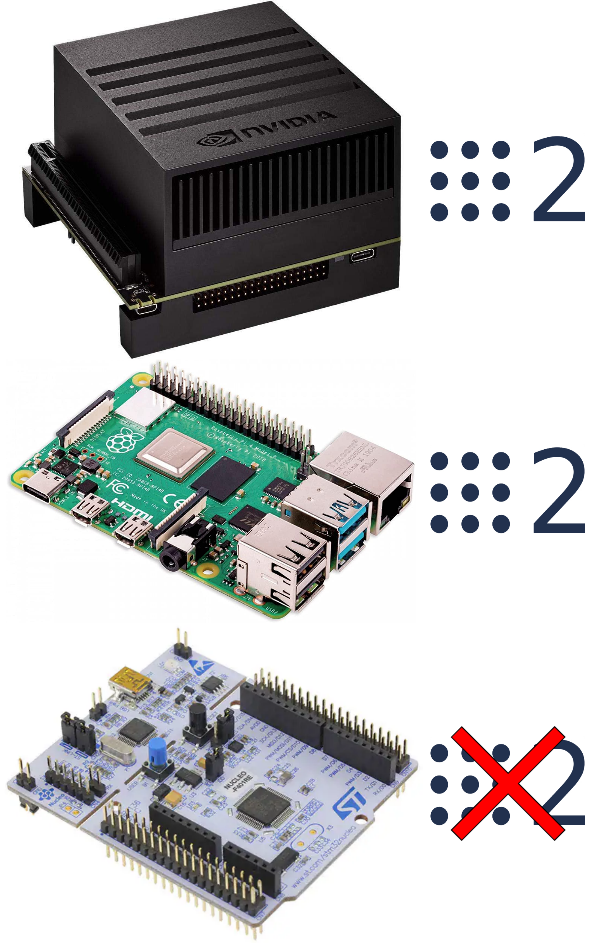
\includegraphics[scale=.19]{why_ros2.png}
      \label{fig:whyros2}
      \caption{STM32 (bottom), Raspberry Pi (middle), and Nvidia Xavier AGX (top)}
		\end{figure}
	\end{columns}
\end{frame}

% --- Main Features ---
\begin{frame}{Main Features}
	As a middleware, it offers the following services to roboticists:
	\begin{itemize}
		\item<1-> \textbg{three inter-process communication (IPC) paradigms}, easy to set up and based on the DDS: \textbg{messages}, \textbg{services} and \textbg{actions};
		\item organization of software packages, allowing for \textbg{redistribution and code reuse}, thanks to the \textbg{colcon} package manager;
		\item<1-> module configuration tools: \textbg{node parameters} and \textbg{launch files};
		\item<1-> integrated \textbg{logging subsystem} (involves both console and log files);
		\item<1-> CLI \textbg{introspection tools} for debugging and testing;
		\item<1-> integration with \textbg{simulators} (e.g. Gazebo) and \textbg{data visualizers} (e.g. RViz);
		\item<2> and much more...
	\end{itemize}
\end{frame}

% --- Flaws ---
\begin{frame}{Flaws}
	\visible<1->{
		\begin{alertblock}{ROS 2 biggest flaws (as of today)}
			The main concerns arise when developing low-level stuff:
			\begin{itemize}
				\item the DDS layer is \textbr{almost completely abstracted}, so some network configurations are impossible;
				\item the internal job scheduling algorithm (namely the \textbr{executor}) is \textbr{not suited for hard real-time applications}.
			\end{itemize}
		\end{alertblock}
	}
	\visible<2>{
		What to do when development gets to a really low level?
		\begin{itemize}
			\item Use \textbg{micro-ROS}: hard real-time ROS 2 on microcontrollers and different communication interfaces.
			\item Hand off stuff to dedicated \textbg{microcontrollers}.
			\item Use something else.
		\end{itemize}
	}
\end{frame}

% --- Job Executors: Events and Callbacks ---
\begin{frame}{Job Executors: Events and Callbacks}
	\begin{figure}
		\centering
		\includesvg[scale=.5]{ROS2_executor_scheme.svg}
		\label{fig:executorscheme}
		\caption{ROS 2 event-based programming paradigm}
	\end{figure}
\end{frame}
\begin{frame}{Job Executors: Events and Callbacks}
	\begin{enumerate}
		\item Middleware functionalities trigger \textbg{(a)synchronous events}.
		\item Events are handled by \textbg{background jobs}, coded in \textbg{callbacks}.
		\item Callbacks are registered into a \textbg{node} when its functionalities are specified (e.g. upon creation).
		\item The workload that a node carries is scheduled and processed by an \textbg{executor}, single- or multi-threaded.
	\end{enumerate}
	\begin{alertblock}{}
		Executors implement a \textbr{round-robin}, \textbr{non-preemptive} scheduling policy that \textbr{always prioritizes timers}.
	\end{alertblock}
	Executors are currently being completely redesigned in Rolling, importing changes from the fixed-priority, preemptive ones of \textbg{micro-ROS}.
\end{frame}
